\chapter{Grundlagen von regulären Ausdrücken}

\section{Äquivalenz verschiedener Modelle}


\begin{figure}[ht]
	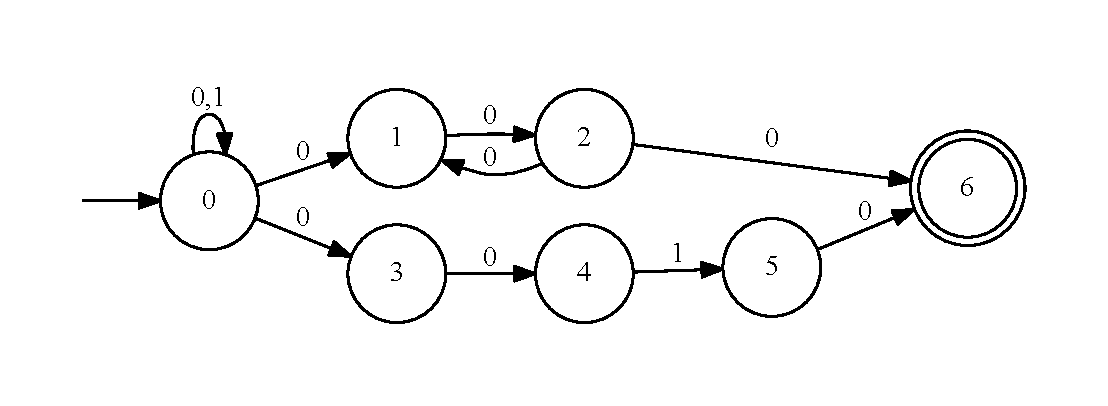
\includegraphics[width=\textwidth]{bilder/nfa_beispiel.pdf}
	\caption{Visuelle Darstellung des NFAs zum regulären Ausdruck \texttt{(0|1)*((00)+|001)0}}
	\label{nfa_beispiel}
\end{figure}

\begin{figure}[ht]
	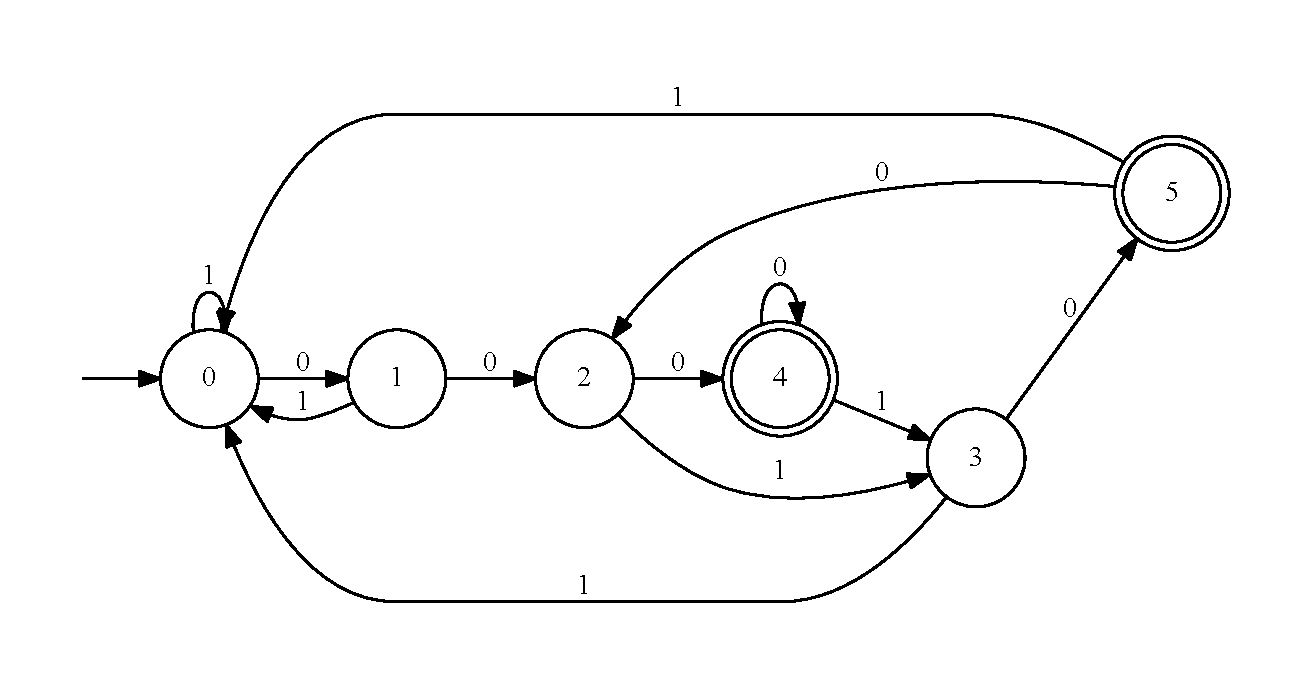
\includegraphics[width=\textwidth]{bilder/dfa_beispiel.pdf}
	\caption{Visuelle Darstellung des DFAs zum regulären Ausdruck \texttt{(0|1)*((00)+|001)0}}
	\label{dfa_beispiel}
\end{figure}

\section{Durchführung eines Musterabgleichs}

\begin{lstlisting}[language=Python,
caption=Durchführung des Musterabgleichs mithilfe eines DFA,
label=dfa_matching]
dfa = [[1, 0],
	[2, 0],
	[4, 3],
	[5, 0],
	[4, 3],
	[2, 0]]
cs = 0
accepting = [4, 5]

word = "010010"

for c in word:
	cs = dfa[cs][int(c)]

if cs in accepting:
	print("Word matches regular expression!")
\end{lstlisting}

\begin{lstlisting}[language=Python,
caption=Durchführung des Musterabgleichs mithilfe eines NFA,
label=nfa_matching]
nfa = [[[0, 1, 3], [0]],
	[[2], []],
	[[1, 6], []],
	[[4], []],
	[[], [5]],
	[[6], []],
	[[], []]]
cs = [0]
accepting = [6]

word = "010010"

for c in word:
	newCs = []
	for s in cs:
		newCs = newCs + nfa[s][int(c)]
	cs = newCs

for s in cs:
	if s in accepting:
		print("Word matches regular expression!")
		break
\end{lstlisting}

\section{Auswahl eines geeigneten Ansatzes}
